\documentclass[tikz,border=5pt]{standalone}
% Standalone TikZ figure: unit circle illustration for the inequalities
%   (1/2) sin(theta) <= (1/2) theta <= (1/2) tan(theta)
% showing sin(theta) <= theta <= tan(theta) for 0 < theta < pi/2.
\usepackage{amsmath}
\usepackage{tikz}
\usetikzlibrary{decorations.pathreplacing,decorations.pathmorphing}

\begin{document}
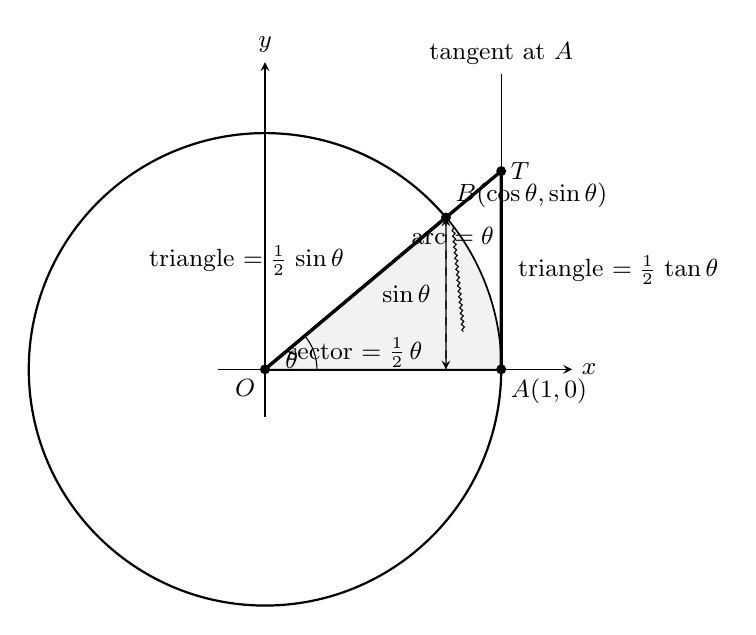
\begin{tikzpicture}[scale=3, >=stealth, every node/.style={font=\small}]
  % angle in degrees (change if desired)
  \def\ang{40}

  % key points
  \coordinate (O) at (0,0);
  \coordinate (A) at (1,0);
  \coordinate (B) at ({cos(\ang)},{sin(\ang)});
  % intersection of ray OB with the tangent line x=1 at A
  \coordinate (T) at (1,{tan(\ang)});

  % axes
  \draw[->] (-0.2,0) -- (1.3,0) node[right] {$x$};
  \draw[->] (0,-0.2) -- (0,1.3) node[above] {$y$};

  % unit circle
  \draw[thick] (O) circle (1);

  % triangle OAB (chord and radii)
  \draw[very thick] (O) -- (B) -- (A) -- cycle;

  % sector (lightly shaded)
  \fill[gray!10] (O) -- (A) arc (0:\ang:1) -- cycle;
  \draw (O) -- (A) (O) -- (B);
  \draw (A) arc (0:\ang:1);

  % small arc mark for theta
  \draw ([shift={(0.22,0)}]0,0) arc (0:\ang:0.22);
  \node at ({0.12*cos(\ang/2)},{0.12*sin(\ang/2)}) {$\theta$};

  % points
  \fill (O) circle (0.6pt) node[below left] {$O$};
  \fill (A) circle (0.6pt) node[below right] {$A(1,0)$};
  \fill (B) circle (0.6pt) node[above right] {$B(\cos\theta,\sin\theta)$};
  \fill (T) circle (0.6pt) node[right] {$T$};

  % vertical showing sin(theta)
  \draw[dashed] (B) -- ({cos(\ang)},0);
  \draw[<->] ({cos(\ang)},0) -- (B) node[midway,left=2pt] {$\sin\theta$};

  % tangent line at A (x=1)
  \draw[thin] (1,-0.05) -- (1,1.25) node[above] {tangent at $A$};

  % larger triangle OAT
  \draw[very thick] (O) -- (T) -- (A);

  % annotations for comparative areas (repositioned to avoid overlap)
  % sector label placed low inside the sector
  \node at (0.38,0.07) {sector $=\tfrac12\,\theta$};
  % small triangle label along OB
  \path (O) -- (B) node[pos=0.52, above left=2pt] {triangle $=\tfrac12\,\sin\theta$};
  % big triangle label to the right of tangent
  \node[anchor=west] at (1.03,{0.5*tan(\ang)}) {triangle $=\tfrac12\,\tan\theta$};

  % optional: arc length label (theta as arc length) moved slightly inward
  \draw[decorate,decoration={snake,amplitude=0.5pt,segment length=2pt}] (0.84,0.16) -- ({cos(\ang)+0.03},{sin(\ang)-0.04});
  \node[above right=1pt] at ({0.74*cos(\ang)},{0.74*sin(\ang)}) {arc $=\theta$};
\end{tikzpicture}
\end{document}